% 图 2.16 磁性核（球）内外磁场分布示意：赤道电流产生，球外似点偶极子，球内场平均向上
\documentclass[tikz,border=5pt]{standalone}
\usetikzlibrary{arrows.meta,decorations.markings}
\usepackage{amsmath}
\usepackage{bm}
\usepackage{fontspec}
\setmainfont{Times New Roman}
\begin{document}
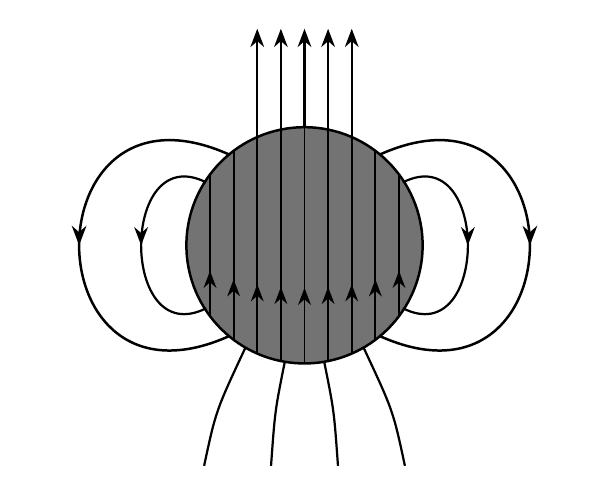
\begin{tikzpicture}[line width=0.8pt,>=Stealth]
\def\R{1.5}
% 球（阴影）
\fill[black!55] (0,0) circle (\R);
% 球内竖直线（下->上，箭头向上表示球内场）
\foreach \x in {-1.2,-0.9,-0.6,-0.3,0,0.3,0.6,0.9,1.2}{
  \pgfmathsetmacro\ye{\R*\R-\x*\x}
  \pgfmathsetmacro\yb{-sqrt(\ye)}
  \pgfmathsetmacro\yt{sqrt(\ye)}
  \draw[line width=0.7pt,postaction={decorate,decoration={markings,
    mark=at position 0.32 with {\arrow[line width=0.7pt]{Stealth}}}}]
    (\x,\yb) -- (\x,\yt);
}
% 球上方出射的竖直场线（5 支，箭头向上）
\foreach \x in {-0.6,-0.3,0,0.3,0.6}{
  \pgfmathsetmacro\yt{sqrt(\R*\R-\x*\x)}
  \draw[line width=0.8pt,->] (\x,\yt) -- (\x,2.75);
}
% 球下方进入的场线（4 支，无箭头）
\foreach \x in {-0.75,-0.25,0.25,0.75}{
  \pgfmathsetmacro\yb{-sqrt(\R*\R-\x*\x)}
  \draw[line width=0.8pt] (\x,\yb) .. controls (1.5*\x,-2.1) .. (1.7*\x,-2.8);
}
% 左右偶极回流线圈（外侧下行）
\draw[line width=0.9pt,postaction={decorate,decoration={markings,
  mark=at position 0.5 with {\arrow[line width=0.9pt]{Stealth}}}}]
  (-0.95,1.15) .. controls (-3.5,2.3) and (-3.5,-2.3) .. (-0.95,-1.15);
\draw[line width=0.9pt,postaction={decorate,decoration={markings,
  mark=at position 0.5 with {\arrow[line width=0.9pt]{Stealth}}}}]
  (0.95,1.15) .. controls (3.5,2.3) and (3.5,-2.3) .. (0.95,-1.15);
\draw[line width=0.8pt,postaction={decorate,decoration={markings,
  mark=at position 0.5 with {\arrow[line width=0.8pt]{Stealth}}}}]
  (-1.25,0.80) .. controls (-2.35,1.35) and (-2.35,-1.35) .. (-1.25,-0.80);
\draw[line width=0.8pt,postaction={decorate,decoration={markings,
  mark=at position 0.5 with {\arrow[line width=0.8pt]{Stealth}}}}]
  (1.25,0.80) .. controls (2.35,1.35) and (2.35,-1.35) .. (1.25,-0.80);
% 球轮廓最后再描一遍（压住内部线端）
\draw[line width=0.9pt] (0,0) circle (\R);
\end{tikzpicture}
\end{document}
